% Complete documentation on the extended LaTeX markup used for Python
% documentation is available in ''Documenting Python'', which is part
% of the standard documentation for Python.  It may be found online
% at:
%
%     http://www.python.org/doc/current/doc/doc.html

%labels
%Sections and subsections \label{sec: }
%Chapters \label{ch: }
%Equations \label{eq: }
%Figures \label{fig: }

% Is latex failing with;
% 'modanuga_user_manual.ind' not found?
% try this command-line
%   makeindex modanuga_user_manual.idx
% To produce the modanuga_user_manual.ind file.

\documentclass{manual}

\usepackage{graphicx}
\usepackage[english]{babel}
\usepackage{datetime}
\usepackage[hang,small,bf]{caption}

%Common definitions for the ANUGA documentation
%

\newcommand{\indexedcode}[1]{\code{#1}\indexascode{#1}}
\newcommand{\indexascode}[1]{\index{#1@{\texttt {#1}}}}
\newcommand{\indexedcodeheader}[1]{{\bigskip \large \bf \code{#1}}\indexascode{#1}\\}
\newcommand{\indexedbold}[1]{\textbf{#1}\index{#1}}
%\newcommand{\anuga}{\textbf{ANUGA}$^{\scriptscriptstyle \copyright}$ v1.0\ }
\newcommand{\anuga}{\textbf{ANUGA} }
%\newcommand{\anugav}[1]{\textbf{ANUGA}$^\copyright$ V#1\ }


\newcommand{\Python}{\textsc{Python}}
\newcommand{\VPython}{\textsc{VPython}}
\newcommand{\pypar}{\textsc{mpi}}
\newcommand{\Metis}{\textsc{Metis}}
\newcommand{\mpi}{\textsc{mpi}}

\newcommand{\hmin}{h_{\min}}

\newcommand{\UU}{\mathbf{U}}
\newcommand{\VV}{\mathbf{V}}
\newcommand{\EE}{\mathbf{E}}
\newcommand{\GG}{\mathbf{G}}
\newcommand{\FF}{\mathbf{F}}
\newcommand{\HH}{\mathbf{H}}
\newcommand{\SSS}{\mathbf{S}}
\newcommand{\nn}{\mathbf{n}}

%\newcommand{\code}[1]{\texttt{#1}}






%Used with \code.
%
\newenvironment{displayedcode}
   {\begin{tabular}{p{0.41cm}l}}
{\end{tabular}}  


\title{\anuga Internal Tools Manual}
\author{Geoscience Australia and the Australian National University}

% Please at least include a long-lived email address;
% the rest is at your discretion.
\authoraddress{Geoscience Australia \\
  Email: \email{ole.nielsen@ga.gov.au}
}

%Draft date

% update before release!
% Use an explicit date so that reformatting
% doesn't cause a new date to be used.  Setting
% the date to \today can be used during draft
% stages to make it easier to handle versions.

\longdate       % Make date format long using datetime.sty
%\settimeformat{xxivtime} % 24 hour Format
\settimeformat{oclock} % Verbose
\date{\today, \ \currenttime}
%\hyphenation{set\_datadir}

\ifhtml
  \date{\today} % latex2html does not know about datetime
\fi

%
% This file is a dummy used if update_anuga_user_manual.py hasn't 
% generated one.
%	
	

% release version; this is used to define the
% \version macro
\release{1.2.1}
 % Get version info - this file may be modified by
                % update_anuga_user_manual.py - if not a dummy
                % will be used.

%\release{1.0}   % release version; this is used to define the
%                % \version macro

\makeindex          % tell \index to actually write the .idx file
\makemodindex       % If this contains a lot of module sections.

\setcounter{tocdepth}{3}
\setcounter{secnumdepth}{3}

%%%%%%%%%%%%%%%%%%%%%%%%%%%%%%%%%%%%%%%%%%%%%%%%%%%%%%%%%%%%%%%%%%%%%%%%%%%%%%%%%%%

\begin{document}
\maketitle

%% This makes the contents more accessible from the front page of the HTML.
%\ifhtml
%  \chapter*{Front Matter\label{front}}
%\fi

%*************************************************
%     LaTeX document
%
%  This is the ANUGA User Manual
%
%  Version 1.0    February, 2006
%
%
%
%  Copyright 2004, 2005, 2006
%  Stephen Roberts, Australian National University
%  Ole Nielsen, Duncan Gray, Jane Sexton, Nick Bartzis, Geoscience Australia
%
%  COPYRIGHT PAGE
%
%
%*************************************************

\vspace*{0.5in}

Copyright \copyright 2004, 2005, 2006 Australian National University and Geoscience Australia. All rights reserved.

Permission to use, copy, modify, and distribute this software for any
purpose without fee is hereby granted under the terms of the GNU
General Public License as published by the Free Software Foundation;
either version 2 of the License, or (at your option) any later
version, provided that this entire notice is included in all copies
of any software which is or includes a copy or modification of this
software and in all copies of the supporting documentation for such
software.

This program is distributed in the hope that it will be useful,
but WITHOUT ANY WARRANTY; without even the implied warranty of
MERCHANTABILITY or FITNESS FOR A PARTICULAR PURPOSE.  See the
GNU General Public License (\url{http://www.gnu.org/copyleft/gpl.html})
for more details.

You should have received a copy of the GNU General Public License
along with this program; if not, write to the Free Software
Foundation, Inc., 59 Temple Place, Suite 330, Boston, MA  02111-1307

This work was produced at Geoscience Australia and the Australian
National University funded by the Commonwealth of Australia. Neither
the Australian Government, the Australian National University,
Geoscience Australia nor any of their employees, makes any warranty,
express or implied, or assumes any liability or responsibility for
the accuracy, completeness, or usefulness of any information,
apparatus, product, or process disclosed, or represents that its use
would not infringe privately-owned rights. Reference herein to any
specific commercial products, process, or service by trade name,
trademark, manufacturer, or otherwise, does not necessarily
constitute or imply its endorsement, recommendation, or favoring by
the Australian Government, Geoscience Australia or the Australian
National University.  The views and opinions of authors expressed
herein do not necessarily state or reflect those of the Australian
Government, Geoscience Australia or the Australian National
University, and shall not be used for advertising or product
endorsement purposes.

This document does not convey a warranty, express or implied,
of merchantability or fitness for a particular purpose.

\begin{center}
  %\vspace{0.5in}
   \anuga

   Manual typeset with \LaTeX
\end{center}

%\vspace{1.5in}
\newpage

\textbf{Credits}:
\begin{itemize}
\item \anuga was developed and is maintained by Stephen Roberts,
  Ole Nielsen, Duncan Gray and Jane Sexton.
\index{ANUGA!credits|textit}  
\end{itemize}

\textbf{License}:
\begin{itemize}
\item \anuga is freely available and distributed under the terms of the GNU General Public Licence.\index{ANUGA!licence|textit}
\end{itemize}


\tableofcontents

%%%%%%%%%%%%%%%%%%%%%%%%%%%%%%%%%%%%%%%%%%%%%%%%%%%%%%%%%%%%%%%%%%%%%%%%%%%%%%%%%%%

\chapter{Internal Tools}


\section{Introduction}

This document describes the tools written for internal \anuga use at Geoscience Australia.

These tools are necessarily ad-hoc in nature and of possibly limited general use.  If
a tool becomes useful to a wider audience it may be moved into the 'ANUGA Tools Manual'.

The tools documented below are:
\begin{itemize}  
  \item acceptance_tests
  \item cmpsww
  \item event_selection
  \item mk_digest
  \item plotcsv
  \item tar_file
  \item update_DVD_images
  \item write_large_files
\end{itemize}   

\pagebreak

\subsection{acceptance_tests}
\label{subsec:acceptance_tests}
\index{acceptance_tests}

This collection of tests is designed to speed up and automate acceptance testing of a
'cluster' of compute servers.  The tests are highly dependent on the installed software
environment, so may have limited use outside Geoscience Australia, though the system
design does lend itself to change.

The suite of tests checks:
\begin{itemize}
  \item installed software, such as python installed packages
  \item availability of NFS mounted filesystems
  \item ability to ssh to each compute node from the master
  \item various aspects of parallel computation
\end{itemize}

The tests are a collection of self-contained acceptance 'testlets' that will be usually
run from a controlling master program, but may be run individually.  This is very useful
when developing a new test, as it can be run by itself until correct.

\subsubsection{Using acceptance_tests}
\label{subsubsec:acceptance_tests_use}

The acceptance tests are designed to be run from the cluster 'master node', so you
must \code{ssh} to that machine.  It is assumed the acceptance tests code suite itself
has been installed on the node it is being run from and other required code has been
installed on all nodes.

Before running the acceptance tests you must prepare some environment variables:

\begin{tabular}{ r l }
PYTHON & Defines the path to the python executable to use for the sub-tests. \\
PYTHONPATH & The path to the \anuga source directory. \\
EQRMPATH & The path to the EQRM source directory.  If not set, EQRM is not tested. \\
\end{tabular}

The first sub-test run dumps the testing environment to the screen as a check.

To run the acceptance tests, do the following:

\begin{verbatim}
export PYTHON=python2.5		# we want to run python 2.5 in the tests
export PYTHONPATH=/home/r-w/sandpit/ga/anuga_core/source/
# EQRMPATH not set
python test_all.py
\end{verbatim}

While the tests are running, you will see the results of each test listed to the 
screen.  Don't worry about catching this output; everything is written to a log file
\code{anuga.log}.

\pagebreak

\subsection{cmpsww}
\label{subsec:cmpsww}
\index{cmpsww.py}

The \code{cmpsww} program is used to compare two SWW files for some approximation
of \emph{equality}.  The user must be able to define what to compare in the two files,
as well as set tolerances for 'how close is close'.

\subsubsection{Using cmpsww}
\label{subsubsec:cmpsww_use}

The usage printed by the program is:

\begin{verbatim}
Usage: cmpsww.py <options> <file1> <file2>
where <options> is zero or more of:
                   -h        print this help
                   -a <val>  set absolute threshold of 'equivalent'
                   -r <val>  set relative threshold of 'equivalent'
                   -g <arg>  check only global attributes specified
                             <arg> has the form <globname>[,<globname>[,...]]
                   -t <arg>  check only timesteps specified
                             <arg> has the form <starttime>[,<stoptime>[,<step>]]
                   -v <arg>  check only the named variables
                             <arg> has the form <varname>[,<varname>[,...]]
and <file1> and <file2> are two SWW files to compare.

The program exit status is one of:
   0    the two files are equivalent
   else the files are not equivalent.
\end{verbatim}

Note that if no globals, variable or timesteps are specified, the program checks
all globals and all variables for all timesteps.

\subsubsection{Bugs}
\label{subsubsec:cmpsww_bugs}

The \code{cmpsww} program is still being developed and needs to change in concert
with the methodology of determining if an SWW file is as expected.

\pagebreak

\subsection{event_selection}
\label{subsec:event_selection}
\index{event_selection.py}

\code{event_selection} is a graphical program used to select earthquake events.

It designed to run under both Windows and Linux.

\subsubsection{Using event_selection}
\label{subsubsec:event_selection_use}

Once you start the \code{event_selection} program you will see:

\begin{figure}[ht]
  \centerline{\fbox{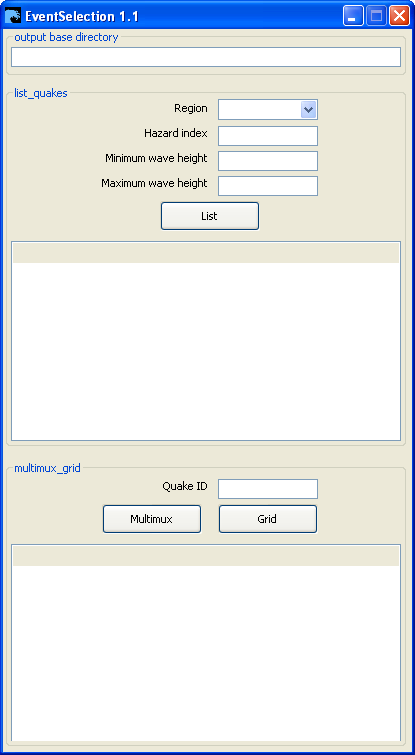
\includegraphics[scale=0.5]{toolgraphics/eventselection/event1.png}}}
  \label{fig:event1}
\end{figure}

Before using the program, you need to set the \emph{output base directory} field at the top
of the window.  The program needs to write
some data files and this field tells the program where to write them.  Just click in the box to
select a directory somewhere in your filesystem.

\pagebreak

We set the directory to \code{C:$\backslash$temp}. 
Next, you need to select the \emph{Region} from the drop-down list:

\begin{figure}[ht]
  \centerline{\fbox{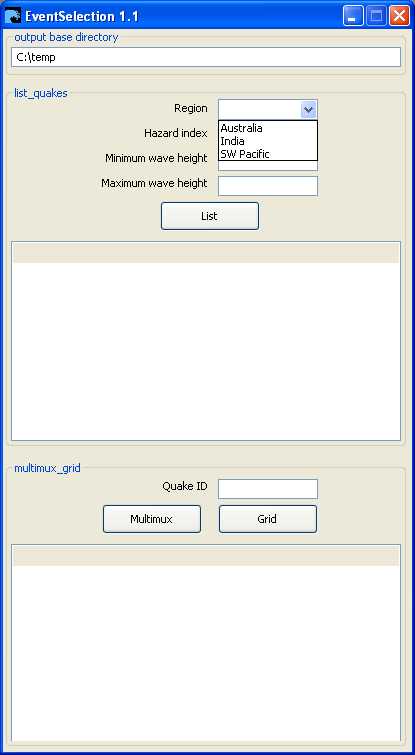
\includegraphics[scale=0.5]{toolgraphics/eventselection/event2.png}}}
  \label{fig:event2}
\end{figure}

At this point you have set the values that will probably never change.  If you close the
program at this point, then the two values set (\emph{base directory} and \emph{Region})
and the three fields below (\emph{Hazard index},
\emph{Minimum wave height} and \emph{Maximum wave height}) will be remembered and restored the 
next time you run the program.  This data is stored in a file \code{event_selection.cfg}
in the \code{event_selection} install directory.

\pagebreak

Now you need to enter data specific to a particular event you are going to model.  Fill
in the \emph{Hazard index} (location in the database of the point where the hazard is measured),
\emph{Minimum wave height} and \emph{Maximum wave height} values
and click on the \emph{List} button:

\begin{figure}[ht]
  \centerline{\fbox{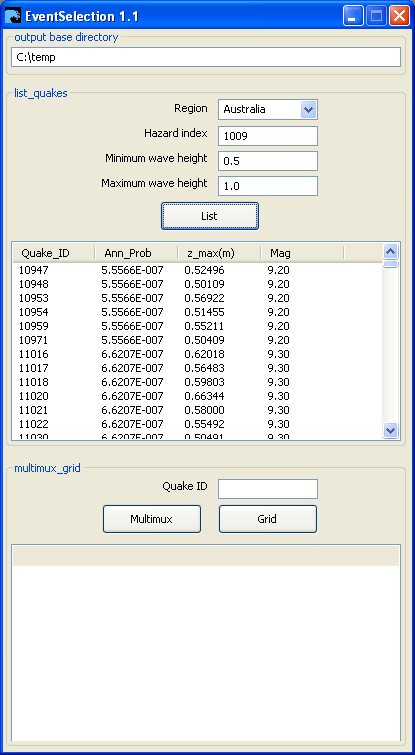
\includegraphics[scale=0.5]{toolgraphics/eventselection/event3.png}}}
  \label{fig:event3}
\end{figure}

\pagebreak

The program has filled the text box below the \emph{List} button with events that satisfy
your listed requirements.  You need to select one of these events, which puts the \emph{Quake_ID}
number into the \emph{Quake_ID} textbox below:

\begin{figure}[ht]
  \centerline{\fbox{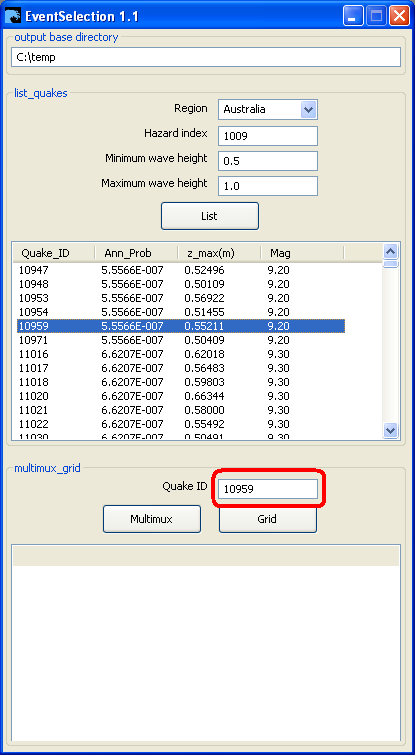
\includegraphics[scale=0.5]{toolgraphics/eventselection/event4.png}}}
  \label{fig:event4}
\end{figure}

\pagebreak

Now you can click on either the \emph{Multimux} or \emph{Grid} buttons.
Clicking on the  \emph{Multimux} button gives us:

\begin{figure}[ht]
  \centerline{\fbox{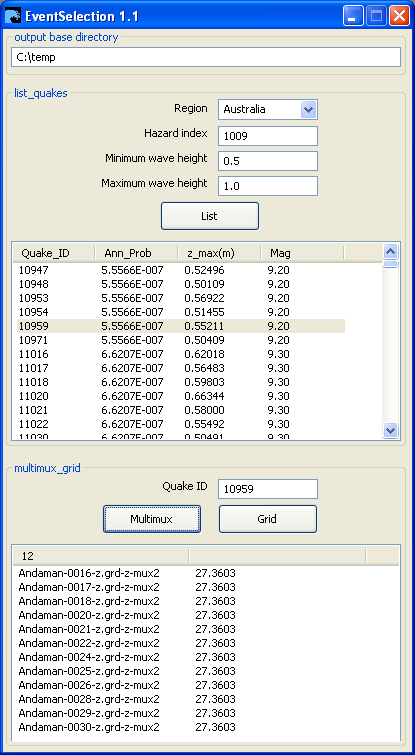
\includegraphics[scale=0.5]{toolgraphics/eventselection/event5.png}}}
  \label{fig:event5}
\end{figure}

If you now look in the output directory \code{C:$\backslash$temp} you will see that two directories have been created:

\begin{verbatim}
10959
Results_Australia_1009_0.50_1.00
\end{verbatim}

The \code{Results_Australia_1009_0.50_1.00} directory contains the \code{fault.xy} and \code{quake_prob.txt}
files used during the calculation of the multimux results.  The \code{Results} directory name contains the 
region name, hazard index and minimum and maximum wave heights in an encoded form.

The \code{10959} directory contains the multimux data for the selected Quake_ID in a file called \code{event_list}.

\pagebreak

The \emph{Grid} button was installed to allow the selection of seafloor deformation grid data.
Clicking on this button shows:

\begin{figure}[ht]
  \centerline{\fbox{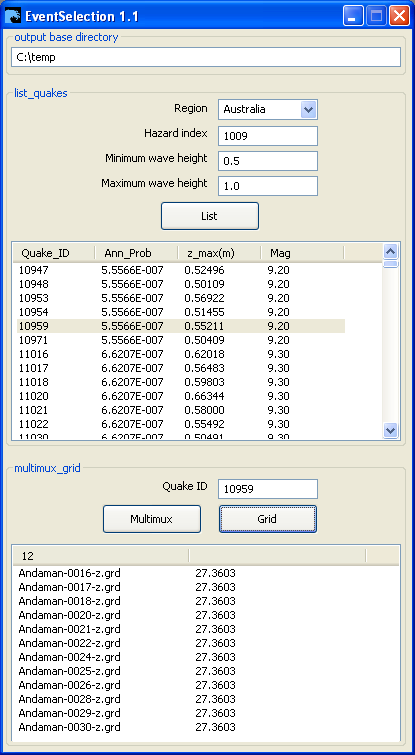
\includegraphics[scale=0.5]{toolgraphics/eventselection/event6.png}}}
  \label{fig:event6}
\end{figure}

and writes some extra files into the \code{Results_Australia_1009_0.50_1.00} directory:

\begin{verbatim}
event_010959.list
faults_010959.params
\end{verbatim}

\pagebreak

The \code{event_010959.list} file contains:

\begin{figure}[ht]
  \centerline{\fbox{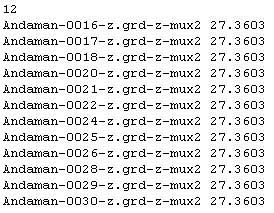
\includegraphics[scale=0.5]{toolgraphics/eventselection/event7.png}}}
  \label{fig:event7}
\end{figure}

The \code{faults_010959.params} file contains:

\begin{figure}[ht]
  \centerline{\fbox{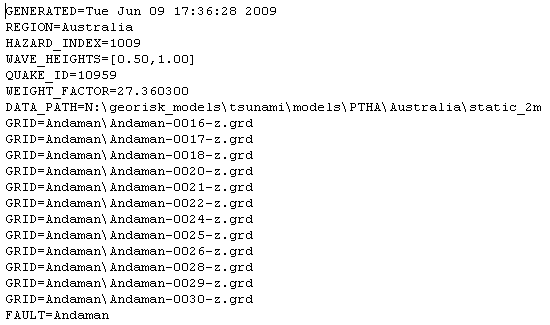
\includegraphics[scale=0.5]{toolgraphics/eventselection/event8.png}}}
  \label{fig:event8}
\end{figure}

\subsection{Installing event_selection}
\label{subsubsec:event_selection_install}

There is an installer program used to install \code{event_selection} on a Windows machine (usually found at 
\code{georisk$\backslash$downloads$\backslash$event_selection}).
The installer is generated by  moving into the \code{installer} directory and right-clicking
on the \code{EventSelection.nsi} file and selecting \code{Compile NSIS script}.  You must have
installed the NSIS package for this to work.  Get it from \url{http://nsis.sourceforge.net/Main_Page}.

Once you have installed \code{event_selection} on your Windows machine you will have a desktop
icon and Start menu entry to start the program with.

Under Linux just execute the \code{event_selection.py} program, either from the console or
from a desktop icon or menu entry you created.

\subsubsection{Requirements}
\label{subsubsec:event_selection_requirements}

Various pieces of python software must be installed before \code{event_selection} can be used.
These are:

\begin{itemize}
  \item wxpython - a python package
  \item NSIS - a Windows installer generator (required if creating a Windows installer)
\end{itemize}

\subsubsection{Bugs}
\label{subsubsec:event_selection_bugs}

The look of \code{event_selection} under Linux is wrong -- it needs to be rewritten using sizers for GUI layout.

\pagebreak

\subsection{mk_digest}
\label{subsec:mk_digest}
\index{mk_digest.py}

\code{mk_digest.py} is a small program used to create an MD5 digest of a file.  The digest string
is written into a file.

This  program is used in the Patong Beach validation file refresh process.

\subsubsection{Using mk_digest}
\label{subsubsec:mk_digest_use}

\begin{verbatim}
usage: mk_digest.py <datafile> <digestfile>
where <datafile>   is the file for which we create a digest string
      <digestfile> is the created file that contains the hex string.
\end{verbatim}

\subsubsection{Installing mk_digest}
\label{subsubsec:mk_digest_install}

Installation is not required, just run the program.

\pagebreak

\subsection{plotcsv}
\label{subsec:plotcsv}
\index{plotcsv.py}

\code{plotcsv} is a GUI program to quickly plot selected columns of one or more CSV files onto a
graph screen.  Once the desired graph is plotted you may save the plot as a picture file.

The program is designed to run under both Windows and Linux.

The CSV files used \emph{must} have column header information as the first line as the column
header values are used during the plotting process.

\subsubsection{Using plotcsv}
\label{subsubsec:plotcsv_use}

Start the program by selecting it from the Start menu or double-clicking on the desktop icon.
You will see the following window:

\begin{figure}[ht]
  \centerline{\fbox{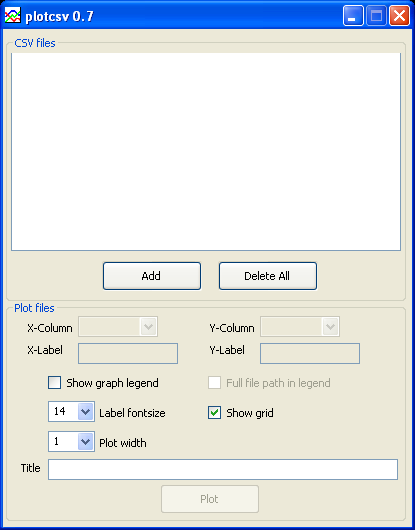
\includegraphics[scale=0.50]{toolgraphics/plotcsv/1.png}}}
  \label{fig:winsetpath1}
\end{figure}

The first thing you must do is select one or more CSV files to plot.  The files you are going to
plot are listed in the textbox at the top of the screen.  There is nothing there because this is
the first time you have run \code{plotcsv}.  Note that \code{plotcsv} will remember the selected files,
as well as other information, when you next start the program.  This files is \code{plotcsv.cfg} and it is 
stored in the \code{plotcsv} install directory.

\pagebreak

This screen shot shows what happens when you click on the \emph{Add} button - you get a file selector 
that lets you choose the CSV files to plot.

\begin{figure}[ht]
  \centerline{\fbox{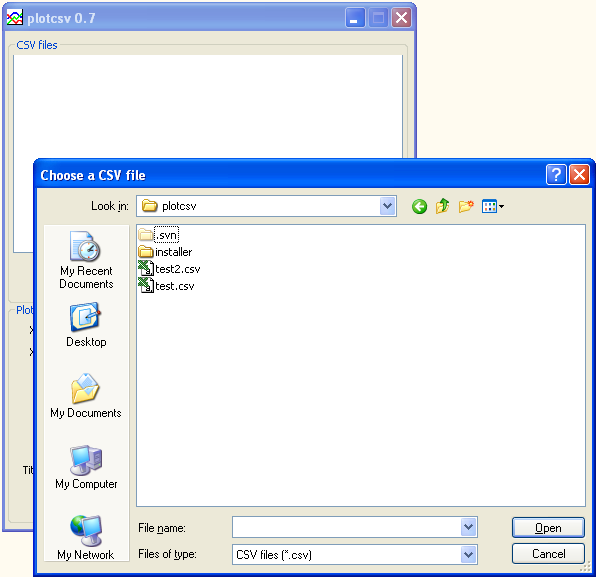
\includegraphics[scale=0.50]{toolgraphics/plotcsv/2.png}}}
  \label{fig:winsetpath1}
\end{figure}

\pagebreak

In this example we selected both \code{test.csv} and \code{test2.csv}.

\begin{figure}[ht]
  \centerline{\fbox{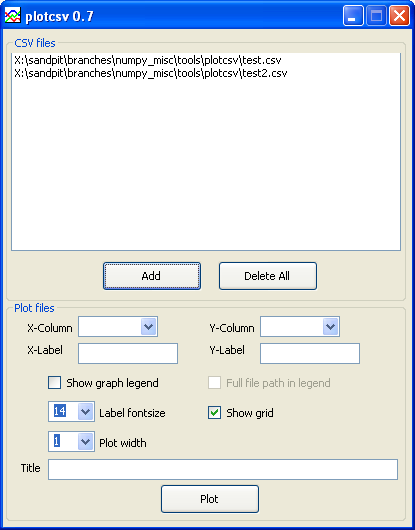
\includegraphics[scale=0.50]{toolgraphics/plotcsv/3.png}}}
  \label{fig:winsetpath1}
\end{figure}

\pagebreak

You must now set the column data to display the X and Y axis of your plot.  The \emph{X-Column}
and \emph{Y-Column} listboxes are used to set which column data to use.  In this example we are
going to plot Stage versus Time, so we select the appropriate columns below:

\begin{figure}[ht]
  \centerline{\fbox{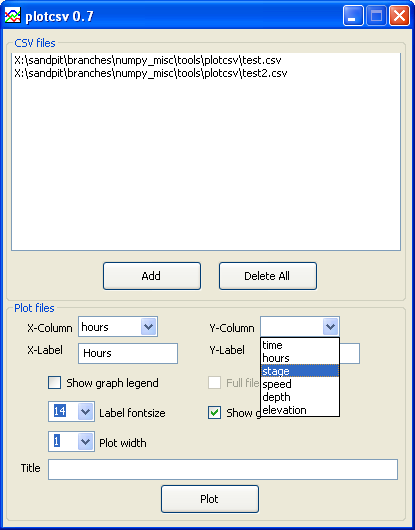
\includegraphics[scale=0.50]{toolgraphics/plotcsv/5.png}}}
  \label{fig:winsetpath1}
\end{figure}

\pagebreak

Note that choosing a column to plot also sets the text in the \emph{X-Label} and \emph{Y-Label}
textboxes.  You can change this text and, in this example, we want to change the stage axis text 
to \emph{Stage (meters)}.  We also add some title text and turn on the graph legend:

\begin{figure}[ht]
  \centerline{\fbox{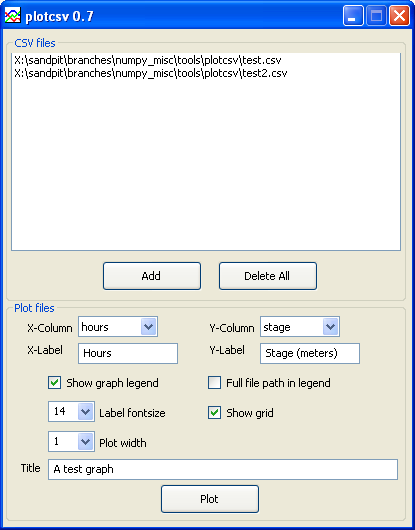
\includegraphics[scale=0.50]{toolgraphics/plotcsv/7.png}}}
  \label{fig:winsetpath1}
\end{figure}

\pagebreak

Finally, once we are ready, we click on the \emph{Plot} button and see our plot:

\begin{figure}[ht]
  \centerline{\fbox{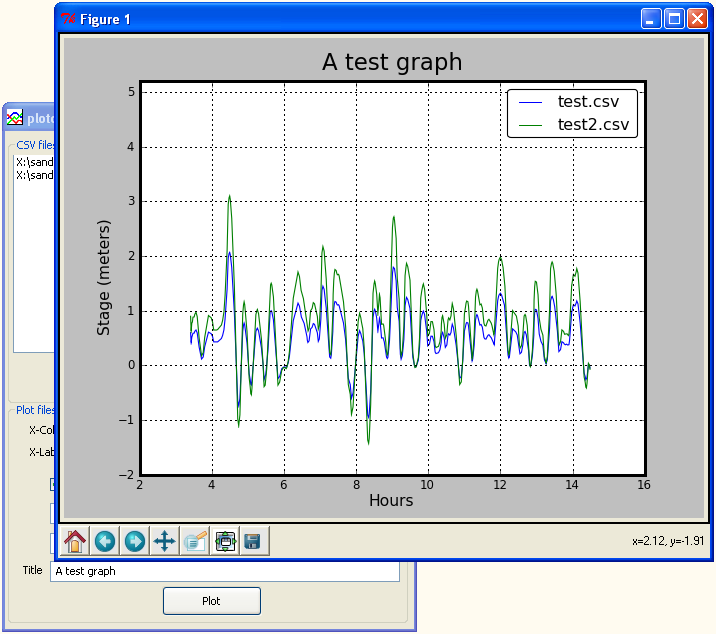
\includegraphics[scale=0.50]{toolgraphics/plotcsv/8.png}}}
  \label{fig:winsetpath1}
\end{figure}

You are free to configure the plot, make it larger, save a picture file, etc.  Closing
the plot window shuts down the application (see Bugs section below).

\pagebreak

\subsubsection{Installing plotcsv}
\label{subsubsec:plotcsv_install}

For Windows execute the \code{plotcsv_X.X.exe} file in \code{N:$\backslash$georisk$\backslash$downloads$\backslash$plotcsv}.
This will install \code{plotcsv} into your \code{C:$\backslash$Program Files} directory and create a desktop icon.

Linux needs no installation, just run the program.

\subsubsection{Building plotcsv for Windows}
\label{subsubsec:plotcsv_build}

The source directory for \code{plotcsv} contains an \code{installer} directory.  Just right-click
on the \code{plotcsv.nsi} file and select "Compile NSIS Script".  You must ihave the NSIS installer installed, of course.
Get it from \url{http://nsis.sourceforge.net/Main_Page}.

\subsubsection{Bugs}
\label{subsubsec:plotcsv_bugs}

The mixture of matplotlib and wxpython isn't successful - you only get one plot and then you must
close the application.  Using the \code{wx_mpl_bars.py} example from
\url{http://eli.thegreenplace.net/2008/08/01/matplotlib-with-wxpython-guis/},
rewrite \code{plotcsv} to have the parameter changes (such as title text) show up immediately in the current plot.

The look of \code{plotcsv} under Linux is wrong -- it needs to be rewritten using sizers for GUI layout.

\pagebreak

\subsection{tar_file}
\label{subsec:tar_file}
\index{tar_file}
\index{tar_file.py}
\index{untar_file.py}

The \code{tar_file.py} program is used to tar and compress a file or directory into a *.tgz file.
We have a python function to do this as we can't use a local \emph{tar} program, as this wouldn't
work under Windows.

The associated \code{untar_file.py} program reverses the above process.

These two programs are used in the Patong Beach validation suite.

\subsubsection{Using tar_file}
\label{subsubsec:tar_file_use}

\begin{verbatim}
tar_file.py <tarfile> <file1> [<file2>, ...]
\end{verbatim}

where \emph{tarfile} is the path to the tar file to create,
and \emph{file?} is the path to a file or  directory to include.

\subsubsection{Using untar_file}
\label{subsubsec:untar_file_use}

\begin{verbatim}
untar_file.py <tarfile> [<output_directory>]
\end{verbatim}

where \emph{tarfile} is the path to the file to untar,
and \emph{output_directory} is the directory to write the results into.

If \emph{output_directory} is not specified then the compressed file is unpacked
into the current directory.

\subsubsection{Installing tar_file}
\label{subsubsec:tar_file_install}

No installation is required, just run the program.

\pagebreak

\subsection{update_DVD_images}
\label{subsec:update_DVD_images}
\index{update_DVD_images.py}

\code{update_DVD_images} is a program used to create the DVD image filesystems that were burnt to DVD
for the 2009 East Coast Tsunami Inundation study.

\subsubsection{Using update_DVD_images}
\label{subsubsec:update_DVD_images_use}

To use the \code{update_DVD_images} program, just execute the program:

\begin{verbatim}
python update_DVD_images.py <name of jurisdiction>
\end{verbatim}

Currently, the jurisdiction names are:

\begin{itemize}
  \item BatemansBay
  \item GoldCoast
  \item Gosford
  \item Hobart
\end{itemize}

So to recreate the GoldCoast DVD image sub_directory, do:

\begin{verbatim}
python update_DVD_images.py goldcoast
\end{verbatim}

Note that the case of the jurisdiction name doesn't matter.

The program will create a new sub-directory with the \emph{formal} jurisdiction name (see below)
in the current directory.  The old jurisdiction sub-directory is deleted first.

\subsubsection{Configuration}
\label{subsubsec:update_DVD_images_config}

Here we discuss how to configure \code{update_DVD_images} to handle a new jurisdiction or
change what files/directories are copied.

In \code{update_DVD_images.py} there are a set of dictionaries that control what is done for each
jurisdiction.

The first dictionary is \code{source_jurisdiction_path} which maps the lowercase jurisdiction name
to the dictionary defining that particular jurisdiction:

\begin{verbatim}
source_jurisdiction_path = {'hobart': hobart_data,
                            'batemansbay': batemans_bay_data,
                            'gosford': gosford_data,
                            'goldcoast': gold_coast_data}
\end{verbatim}

If you create a new jurisdiction, you need to add another line to the above dictionary.

\pagebreak

In the case of the GoldCoast jurisdiction, we see that the dictionary for the GoldCoast is 
\code{gold_coast_data}:

\begin{verbatim}
gold_coast_data = \
{'jurisdiction':    'GoldCoast',        # jurisdiction name

 # paths to various source directories
 'data_src_path':   'data/queensland/gold_coast_tsunami_scenario_2009/anuga',
 'arcgis_src_path': 'data/queensland/gold_coast_tsunami_scenario_2009/ArcGIS',
 'proj_src_path':   'sandpits/lfountain/anuga_work/production/gold_coast_2009',

 # paths to destination directories (under 'jurisdiction' root)
 'data_dst_path':   'anuga',
 'proj_dst_path':   'project',
 'arcgis_dst_path': 'ArcGIS',

 # copy or create whole directories
 'make_dst_dirs':   ['outputs'],
 'copy_data_dirs':  ['boundaries'],

 # copy 'data' files or directories
 'copy_data_files': ['outputs/Event1_HAT', 'outputs/Event1_MSL',
                     'outputs/Event2_HAT', 'outputs/Event2_MSL',
                     'outputs/Event3_HAT', 'outputs/Event3_MSL'
                    ],

 # copy 'project' files or directories
 'copy_proj_files': ['build_elevation.py', 'export_results_max.py',
                     'get_runup.py', 'project.py', 'run_model.py',
                     'setup_model.py', 'build_urs_boundary.py',
                     'combine_gauges.py', 'get_timeseries.py',
                     'run_multiple_events.py'
                    ],

 # copy 'arcgis' files or directories
 'copy_arc_files':  ['MainBeach.mxd', 'SurfersParadise.mxd', 'GoldCoast.mxd',
                     'PalmBeach.mxd', 'Collangatta.mxd'
                    ]
}
\end{verbatim}

The first key is \code{jurisdiction}, which maps to a string defining the jurisdiction formal name. 
This name is used to create the output DVD staging directory.

\begin{verbatim}
'jurisdiction':    'GoldCoast',
\end{verbatim}

The next three key values define the complete paths to source directories in the production filesystem:

\begin{verbatim}
# paths to various source directories
'data_src_path':   'data/queensland/gold_coast_tsunami_scenario_2009/anuga',
'arcgis_src_path': 'data/queensland/gold_coast_tsunami_scenario_2009/ArcGIS',
'proj_src_path':   'sandpits/lfountain/anuga_work/production/gold_coast_2009',
\end{verbatim}

\pagebreak

These key values are used along with a master path variable defined earlier in
\code{update_DVD_images.py} to create the complete paths to source directories:

\begin{verbatim}
main_path = '/nas/gemd/georisk_models/inundation'
\end{verbatim}

For example, the full path to the 'data' source directory would be:

\begin{verbatim}
data_src_path = os.path.join(main_path, j_dict['data_src_path'])
\end{verbatim}

where \code{j_dict} would be a reference to the jurisdiction dictionary controlling the
process (\code{gold_coast_data} in this case).

The next three definitions define the names of output directories in the staging directory:

\begin{verbatim}
# paths to destination directories (under 'jurisdiction' root)
'data_dst_path':   'anuga',
'proj_dst_path':   'project',
'arcgis_dst_path': 'ArcGIS',
\end{verbatim}

These three names are combined with the current directory and the jurisdiction
staging directory name to produce the full path to output directories:

\begin{verbatim}
data_dst_path = os.path.join(os.getcwd(), j_name, j_dict['data_dst_path'])
proj_dst_path = os.path.join(os.getcwd(), j_name, j_dict['proj_dst_path'])
arcgis_dst_path = os.path.join(os.getcwd(), j_name, j_dict['arcgis_dst_path'])
\end{verbatim}

Note that \code{j_name} is the jurisdiction name.  So in this case, we would
create the output directories:

\begin{verbatim}
./GoldCoast/anuga               # data directory
./GoldCoast/project             # project files directory
./GoldCoast/ArcGIS              # ArcGIS files
\end{verbatim}

The next two key values define the names of empty directories to create or names of
complete directories to copy to the \code{data_dst_path} directory:

\begin{verbatim}
# copy or create whole directories
'make_dst_dirs':   ['outputs'],
'copy_data_dirs':  ['boundaries'],
\end{verbatim}

The values here are lists of one or more directories to create or copy.  If there are no directories
to create/copy, just use an empty list.

\pagebreak

Next, we define which individual files we copy to the destination data directory:

\begin{verbatim}
# copy 'data' files or directories
'copy_data_files': ['outputs/Event1_HAT', 'outputs/Event1_MSL',
                    'outputs/Event2_HAT', 'outputs/Event2_MSL',
                    'outputs/Event3_HAT', 'outputs/Event3_MSL'],
\end{verbatim}

Again we have a list of files to copy.  Note that we must specify the path following the
\code{data_dst_path} variable (\code{anuga} in this case), so we specify the directory under 
\code{anuga} and then the source file (or directory).  Also note that we can copy a simple file
or complete directory here.

You \emph{must} create each target directory as an empty directory before copying files.
That is why \code{outputs} appears in the \code{make_dst_dirs} key-value definition above.

Similarly, we now define 'project' files to copy:

\begin{verbatim}
 # copy 'project' files or directories
 'copy_proj_files': ['build_elevation.py', 'export_results_max.py',
                     'get_runup.py', 'project.py', 'run_model.py',
                     'setup_model.py', 'build_urs_boundary.py',
                     'combine_gauges.py', 'get_timeseries.py',
                     'run_multiple_events.py'],
\end{verbatim}

These files (or directories) will be copied from the path defined in the \code{proj_src_path}
variable to the path defined in the \code{proj_dst_path} variable.

Finally, we define 'arcgis' files or directories to copy:

\begin{verbatim}
# copy 'arcgis' files or directories
'copy_arc_files':  ['MainBeach.mxd', 'SurfersParadise.mxd', 'GoldCoast.mxd',
                    'PalmBeach.mxd', 'Collangatta.mxd']
\end{verbatim}

These files (or directories) will be copied from the path defined in the \code{arcgis_src_path}
variable to the path defined in the \code{arcgis_dst_path} variable.

\subsubsection{extra_files}
\label{subsubsec:update_DVD_images_extra_files}

In the same directory as \code{update_DVD_images} there must be a directory \code{extra_files}.
This directory contains 'scaffolding' files that must exist on the DVD as well as jurisdiction-specific
files that may be modifications of project files that replace those files on the DVD.

All files in the \code{extra_files} directory are copied to each jurisdiction DVD staging directory.
All top-level directories that \emph{aren't} named for a jurisdiction are also copied to each
staging directory.

Each directory named for a jurisdiction will be copied to the staging directory
if the directory has the same name as the jurisdiction staging directory we are creating.
This jurisdiction directory would normally contain jurisdiction-specific scaffolding
files, such as \code{index.html}, etc, as well as modified project files.

\pagebreak

\subsection{update_lic_checksum}
\label{subsec:update_lic_checksum}
\index{update_lic_checksum.py}
\index{create_lic_file.py}

The \code{update_lic_checksum} program is used to update all licence files (\code{*.lic}) in
a filesystem sub_tree.

The \code{create_lic_file} program is used to create a licence file that controls one or more
data files.

\subsubsection{Using update_lic_checksum}
\label{subsubsec:update_lic_checksum_use}

The program is used:

\begin{verbatim}
update_lic_checksum.py [-m <lic_mask>] <directory>
\end{verbatim}

where \emph{directory} is the path to the sub_directory containing licence files to update.
Normally, \code{update_lic_checksum} would search for and update all \code{*.lic} files.  If you
want to update licence files that have a filename form of \code{*.txt} then use the
\code{-m *.txt} option.

Note that the licence files being updated must contain well-formed XML data.

\subsubsection{Using create_lic_file}
\label{subsubsec:create_lic_file_use}

\code{create_lic_file} is a program used to create licence files from scratch.  It is used so:

\begin{verbatim}
usage: create_lic_file.py <options> <lic_file> [<filename> ...]
where <options>  is zero or more of:
                  --author <name>
                  -w <name>             - name of the author
                  --publishable [Yes|No]
                  -p [Yes|No]           - is document publishable
                  --accountable <name>
                  -a <name>             - name of person accountable for file
                  --source <string>
                  -s <string>           - source of controlled file
                  --owner <name>
                  -o <name>             - IP owner name
                  --info <string>
                  -i <string>           - IP extra information
      <lic_file> is the name of the licence file to create.
      <filename> is one or more files to control.
\end{verbatim}

If the file to be created (\emph{lic_file}) already exists, the program aborts; it will
not overwrite any existing file.

\pagebreak

You must use the options to specify author name, etc.  If these are not overridden the 
generated licence file will contain default values. For example, if you did this:

\begin{verbatim}
python create_lic_file.py test.lic README
\end{verbatim}

then the output file \code{test.lic} would contain:

\begin{verbatim}
<?xml version='1.0' encoding='iso-8859-1'?>
<ga_license_file>
  <metadata>
    <author>rwilson</author>
  </metadata>
  <datafile>
    <filename>README</filename>
    <checksum>1387779554</checksum>
    <publishable>Y</publishable>
    <accountable>rwilson</accountable>
    <source>Generated by ANUGA development team</source>
    <IP_owner>Geoscience Australia</IP_owner>
    <IP_info>For use with the ANUGA test suite</IP_info>
  </datafile>
</ga_license_file>
\end{verbatim}

In particular, the \emph{author} and \emph{accountable} values are defaulted with
the username from the environment.

Note the default values for these fields:

\begin{verbatim}
<publishable>Y</publishable>
<source>Generated by ANUGA development team</source>
<IP_owner>Geoscience Australia</IP_owner>
<IP_info>For use with the ANUGA test suite</IP_info>
\end{verbatim}

\pagebreak

\subsection{write_large_files}
\label{subsec:write_large_files}
\index{write_large_files}
\index{rwi_big_file.py}
\index{rwil_big_file.py}
\index{rwi4_big_file.py}

This program is actually a suite of programs used to exercise the NetCDF file I/O code.

The NetCDF I/O model has three models of the way data is written:
\begin{itemize}
  \item The 'classic' model
  \item The 'large' model
  \item The 'NetCDF4' model
\end{itemize}

The \emph{classic} model is usually dismissed as the '2GiB limit' model, but this
is an over-simplification.  Chunks of data wriiten to a file in one write will contain
an offset to the next related chunk 'upstream' in the file.  This offset has a 2GiB
limit, hence the '2Gib' oversimplification.

The \emph{long} model relaxes some of the limits in the \emph{classic} model.

The \emph{NetCDF4} model allows much larger datasets to be written to a file, along
with compression, more than one unlimited dimension, etc.

Some effort is made to simulate the way an \anuga program would write data.  In  particular,
the variables written are interleaved in the way \anuga would write them.

Also, each data value written to the file is a floating point number which encodes
variable number, variable 'slice' and index into each slice.  This is to ensure that 
each variable value written is unique and to allow for checking that what we read is what we wrote.

\subsubsection{Using write_large_files}
\label{subsubsec:write_large_files_use}

There are three programs in the \code{write_large_files} suite:

\begin{tabular}{ l l }
  rwi_big_file.py & writes using the \emph{classic} model \\
  rwil_big_file.py & writes using the \emph{large} model \\
  rwi4_big_file.py & writes using the \emph{NetCDF4} model \\
\end{tabular}

Each of the three programs is used in the same way:

\begin{verbatim}
Usage: write_large_files <opts> <varsize> [<numvars>]

where <varsize> is a number followed by an optional modifier:
                    1024M or 4G
                the assumed modifier if none is given is 'M'.
  and <numvars> is the number of variables of the above size
                    to write.  If not supplied, 1 is assumed.
                    There can be at most 100 variables.
  and <opts>    is zero or more of:
                    -c s    close & open the output file after
                            each variable slice is read/written,
                    -t rf   time the complete file read,
                    -t wf   time the complete file write,
\end{verbatim}

For instance, if we wanted to write a 3GiB 'large' file containing 6 variables we would do:

\begin{verbatim}
python rwil_big_file.py 512M 6
\end{verbatim}

\subsubsection{Installing write_large_files}
\label{subsubsec:write_large_files_install}

No installation is necessary, just execute the programs.

\subsubsection{Bugs}
\label{subsubsec:write_large_files_bugs}

Instead of having three files, one to test each NetCDF model, just add an extra option to 
a single program:
\begin{verbatim}
  -c    classic model (default)
  -l    large model
  -4    NetCDF4 model
\end{verbatim}

%begin{latexonly}
%\renewcommand{\indexname}{Index}
%end{latexonly}
%\input{\jobname.ind}            % Index

\end{document}
